\setlength{\columnsep}{3pt}
\begin{flushleft}

\bigskip
\begin{itemize}
	\item \textbf{lsblk}: Lists information about all available block devices.
	
	\bigskip
	\begin{tcolorbox}[breakable,notitle,boxrule=-0pt,colback=pink,colframe=pink]
		\color{black}
		\fontdimen2\font=1em
		Syntax: lsblk
		\fontdimen2\font=4pt
	\end{tcolorbox}
	Eg:
	\begin{figure}[h!]
		\centering
		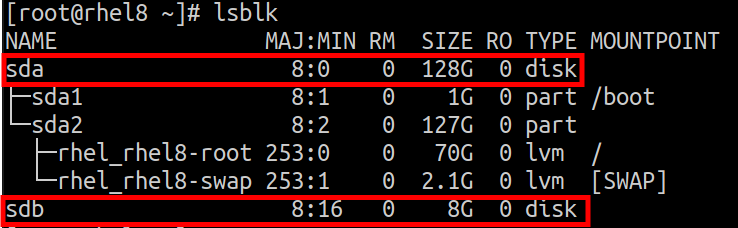
\includegraphics[scale=0.45]{content/chapter8/images/lsblk.png}
		\caption{lsblk command output}
		\label{fig:lsblk}
	\end{figure}
	
	\item \textbf{fdisk -l}: Display more detailed information about all disk drives.
	\bigskip
	\begin{tcolorbox}[breakable,notitle,boxrule=-0pt,colback=pink,colframe=pink]
		\color{black}
		\fontdimen2\font=1em
		Syntax: fdisk -l
		\fontdimen2\font=4pt
	\end{tcolorbox}
	Eg:
	\begin{figure}[h!]
		\centering
		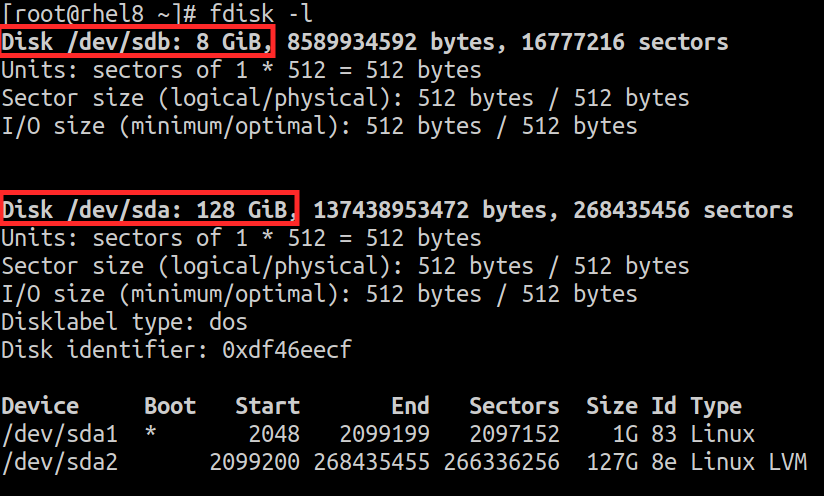
\includegraphics[scale=0.45]{content/chapter8/images/fdisk.png}
		\caption{"fdisk -l" command output}
		\label{fig:fdisk}
	\end{figure}
	
	\item \textbf{du}: Estimate file space usage.
	\bigskip
	\begin{tcolorbox}[breakable,notitle,boxrule=-0pt,colback=pink,colframe=pink]
		\color{black}
		\fontdimen2\font=1em
		Syntax: du [option] [file/folder]
		\fontdimen2\font=4pt
	\end{tcolorbox}
	Eg: 
	\begin{tcolorbox}[breakable,notitle,boxrule=-0pt,colback=black,colframe=black]
		\color{green}
		\fontdimen2\font=1em
		\# du /home
		\fontdimen2\font=4pt
	\end{tcolorbox}

	Options with \textbf{du} command:
	
	\begin{itemize}
		\item \textbf{-sh}: Display only a total for each argument in human readable format.
		\begin{tcolorbox}[breakable,notitle,boxrule=-0pt,colback=pink,colframe=pink]
			\color{black}
			\fontdimen2\font=1em
			Syntax: du -sh [folder/file]
			\fontdimen2\font=4pt
		\end{tcolorbox}
		Eg:
		\begin{tcolorbox}[breakable,notitle,boxrule=-0pt,colback=black,colframe=black]
			\color{green}
			\fontdimen2\font=1em
			\# du -sh /home
			\newline
			\color{white}
			16K	/home
			\fontdimen2\font=4pt
		\end{tcolorbox}
		\bigskip
		\bigskip		
\end{itemize}
	
\end{flushleft}

\newpage

